\begin{tabular}{M{6.5cm}M{11cm}}
	\textbf{LỚP CÔ THẢO - THẦY SANG}& \textbf{ĐỀ ÔN TẬP KIỂM TRA GIỮA HỌC KÌ 1}\\
	\textbf{MÃ ĐỀ: 001}& \textbf{Bài thi môn: VẬT LÝ 12}\\
	\textit{(Đề trường Nguyễn Khuyến \newline Bình Dương năm học 2024 -2025)}& \textit{Thời gian làm bài: 50 phút, không kể thời gian phát đề}
	
	\noindent\rule{4cm}{0.8pt} \\
\end{tabular}
\setcounter{section}{0}
\section{Câu trắc nghiệm nhiều phương án lựa chọn}
\textit{Thí sinh trả lời từ câu 1 đến câu 18. Mỗi câu hỏi thí sinh chọn một phương án}
\setcounter{ex}{0}
\Opensolutionfile{ans}[ans/G12-1-TN]
% ===================================================================
\begin{ex}
	Một nhiệt kế thể tích không đổi hiển thị nhiệt độ $\SI{0}{\celsius}$ và $\SI{100}{\celsius}$ tương ứng với các áp suất $\SI{50}{\centi\meter Hg}$ và $\SI{90}{\centi\meter Hg}$. Biết nhiệt độ đọc được là hàm bậc nhất của áp suất. Khi áp suất thủy ngân là $\SI{60}{\centi\meter Hg}$ thì nhiệt độ đọc được bằng
	\choice
	{$\SI{35}{\celsius}$}
	{$\SI{30}{\celsius}$}
	{$\SI{20}{\celsius}$}
	{\True $\SI{25}{\celsius}$}
	\loigiai{
		$$\dfrac{t-t_b}{t_s-t_b}=\dfrac{p-p_b}{p_s-p_b}\Leftrightarrow \dfrac{t-0}{100-0}=\dfrac{60-50}{90-50}\Rightarrow t=\SI{25}{\celsius}.$$
	}
\end{ex}
% ===================================================================
\begin{ex}
	Chọn phát biểu \textbf{sai}? Sự bay hơi của một khối chất lỏng
	\choice
	{phụ thuộc vào diện tích mặt thoáng, diện tích mặt thoáng càng lớn thì sự bay hơi xảy ra càng nhanh}
	{xảy ra ở nhiệt độ bất kỳ}
	{phụ thuộc vào nhiệt độ, nhiệt độ càng cao sự bay hơi xảy ra càng nhanh}
	{\True phụ thuộc vào độ ẩm của không khí trên mặt thoáng, độ ẩm càng lớn thì sự bay hơi xảy ra càng nhanh}
	\loigiai{
		Độ ẩm càng bé thì sự bay hơi xảy ra càng nhanh.
	}
\end{ex}
% ===================================================================
\begin{ex}
	Để diệt trừ các bào tử nấm và kích thích quá trình nảy mầm của hạt giống lúa, người nông dân đã sử dụng một kinh nghiệm dân gian là ngâm chúng vào trong nước ấm theo công thức "hai sôi, ba lạnh". Tức là nước ấm ở nhiệt độ $T_{\mathrm{A}}\left(\si{\celsius}\right)$ sẽ được tạo ra bằng cách pha hai phần nước sôi $\left(\SI{100}{\celsius}\right)$ với ba phần nước lạnh $T_{\mathrm{L}}\left(\si{\celsius}\right)$. Chọn biểu thức đúng.
	\choice
	{$T_{\mathrm{A}}=\dfrac{200+3 T_{\mathrm{L}}}{2}$}
	{$T_{\mathrm{A}}=\dfrac{200+2 T_{\mathrm{L}}}{3}$}
	{\True $T_{\mathrm{A}}=\dfrac{200+3 T_{\mathrm{L}}}{5}$}
	{$T_{\mathrm{A}}=\dfrac{100+3 T_{\mathrm{L}}}{2}$}
	\loigiai{
		$$T_{\mathrm{A}}=\dfrac{m_scT_s+m_LcT_L}{m_sc+m_Lc}=\dfrac{2\cdot100+3T_L}{2+3}=\dfrac{200+3T_L}{5}.$$
	}
\end{ex}
% ===================================================================
\begin{ex}
	Nhiệt hóa hơi riêng có đơn vị đo là	
	\choice
	{$\si{\joule\cdot\kilogram/\kelvin}$}
	{$\si{\joule/\kilogram\cdot\kelvin}$}
	{\True $\si{\joule/\kilogram}$}
	{$\si{\joule}$}
	\loigiai{}
\end{ex}
% ===================================================================
\begin{ex}
	Chọn đáp án \textbf{sai}? Nhiệt hóa hơi riêng của chất lỏng phụ thuộc vào
	\choice
	{\True khối lượng của khối chất lỏng đó}
	{bản chất của khối chất lỏng đó (chất lỏng đó là chất gì, là nước hay dầu,\dots)}
	{nhiệt độ sôi của khối chất lỏng đó}
	{áp suất bề mặt của khối chất lỏng đó}
	\loigiai{}
\end{ex}
% ===================================================================
\begin{ex}
	Khi thép đang nóng chảy được làm nguội nhanh về nhiệt độ phòng sẽ giúp tăng độ cứng cho thép và cách làm như vậy được gọi là tôi thép. Người ta có thể sử dụng nước để làm hạ nhiệt độ nhanh cho thép đang nóng đỏ vì
	\choice
	{sử dụng nước là do thói quen vì thật ra có thể để thép nóng đỏ trong không khí thì thép cũng hạ nhanh về nhiệt độ phòng}
	{nhiệt độ nóng chảy của nước thấp hơn nhiều so với của thép}
	{\True nhiệt dung riêng của nước cao hơn nhiều so với của thép trong khi đó nhiệt độ sôi của nước lại thấp hơn nhiều so với nhiệt độ nóng chảy của thép}
	{nước có khả năng bốc hơi rất nhanh khi gặp kim loại nóng}
	\loigiai{}
\end{ex}
% ===================================================================
\begin{ex}
	Biểu thức diễn tả đúng độ biến thiên nội năng $\Delta U$ của chất khí trong quá trình chất khí vừa nhận nhiệt $Q$ vừa nhận công $A$ là?
	\choice
	{$\Delta U=A+Q$; $Q>0$; $A<0$}
	{$\Delta U=Q$; $Q>0$}
	{$\Delta U=Q+A$; $Q<0 $; $A>0$}
	{\True $\Delta U=Q+A$; $Q>0 $; $A>0$}
	\loigiai{}
\end{ex}
% ===================================================================
\begin{ex}
	Nước là chất có X lớn hơn nhiều so với các chất lỏng thông thường khác. Nhờ đó, nước có vai trò quan trọng đối với đời sống con người. Khoảng $\SI{70}{\percent}$ bề mặt của Trái Đất được bao phủ bởi nước. Nhờ có X lớn nên lượng nước này có thể hấp thụ lượng nhiệt khổng lồ của năng lượng mặt trời mà vẫn giữ cho nhiệt độ của bề mặt Trái Đất tăng không nhanh và không nhiều, tạo điều kiện thuận lợi cho sự sống của con người và các sinh vật khác. Cũng nhờ có X lớn mà nước biển nóng lên và nguội đi chậm hơn các vùng đất xung quanh. Do sự ổn định này của nhiệt độ nước biển mà các đảo và các vùng đất ven biển có khí hậu tương đối ôn hoà, thích hợp với con người. Cũng nhờ có X mà nước thường được dùng trong các thiết bị làm mát của động cơ nhiệt. Cụm từ tương ứng với X là
	\choice
	{nhiệt hóa hơi riêng}
	{nhiệt nóng chảy riêng}
	{khối lượng riêng}
	{\True nhiệt dung riêng}
	\loigiai{}
\end{ex}
% ===================================================================
\begin{ex}
	Khi làm muối, người ta đã dựa vào hiện tượng nào của nước?
	\choice
	{Sự sôi}
	{\True Bay hơi}
	{Đông đặc}
	{Ngưng tụ}
	\loigiai{}
\end{ex}
% ===================================================================
\begin{ex}
	Nhiệt hoá hơi riêng của một chất là nhiệt lượng cần cung cấp để $\SI{1}{\kilogram}$ chất đó
	\choice
	{hoá hơi hoàn toàn}
	{hoá hơi}
	{\True hoá hơi hoàn toàn ở nhiệt độ sôi}
	{bay hơi hết}
	\loigiai{}
\end{ex}
% ===================================================================
\begin{ex}
	Cho nhẹ nhàng vài viên đá vào một cốc nước. Sau một lúc ta thấy bên ngoài thành cốc có các giọt nước nhỏ li ti bám vào. Hiện tượng đó là do
	\choice
	{nước trong cốc thấm ra}
	{hơi nước trong không khí gặp lạnh ngưng kết lại}
	{\True hơi nước trong không khí gặp lạnh ngưng tụ}
	{nước trong cốc bay hơi và ngưng tụ lại}
	\loigiai{}
\end{ex}
% ===================================================================
\begin{ex}
	Ở thể khí, các phân tử ở (1) \dots Lực tương tác giữa các phân tử (2) \dots (trừ truờng hợp chúng va chạm nhau) nên các phân tử chuyển động hoàn toàn (3) \dots Do đó, khối chất khí không có (4) \dots.
	\choice
	{(1) gần nhau, (2) rất yếu, (3) trật tự, (4) hình dạng và thể tích riêng}
	{(1) gần nhau, (2) rất mạnh, (3) hỗn loạn, (4) hình dạng và thể tích riêng}
	{(1) xa nhau, (2) rất yếu, (3) hỗn loạn, (4) khối lượng và hình dạng}
	{\True (1) xa nhau, (2) rất yếu, (3) hỗn loạn, (4) hình dạng và thể tích riêng}
	\loigiai{}
\end{ex}
% ===================================================================
\begin{ex}
	Gọi lực liên kết giữa các phân tử trong chất rắn, chất lỏng, chất khí lần lượt là $F_{1}$, $F_{2}$, $F_{3}$ thì
	\choice
	{$F_{1}<F_{2}=F_{3}$}
	{$F_{1}=F_{2}=F_{3}$}
	{$F_{1}>F_{2}=F_{3}$}
	{\True $F_{1}>F_{2}>F_{3}$}
	\loigiai{}
\end{ex}
% ===================================================================
\begin{ex}
	Dùng một ca múc nước ở thùng chứa nước A có nhiệt độ $t_{\mathrm{A}}=\SI{20}{\celsius}$ và ở thùng chứa nước B ở nhiệt độ $t_{\mathrm{B}}=\SI{80}{\celsius}$ rồi đổ vào thùng nước C. Biết rằng trước khi đổ, trong thùng chứa nước C đã có sẵn một lượng nước ở nhiệt độ $t_{\mathrm{C}}=\SI{40}{\celsius}$ và bằng tổng số ca nước vừa mới đổ thêm vào nó. Bỏ qua sự trao đổi nhiệt với môi trường, với bình chứa và ca múc nước. Để có nhiệt độ nước ở thùng C là $\SI{50}{\celsius}$ thì số ca nước phải múc ở mỗi thùng A và B lần lượt là
	\choice
	{$3n$ ca và $2n$ ca}
	{\True $n$ ca và $2n$ ca}
	{$2n$ ca và $n$ ca}
	{$n$ ca và $3n$ ca}
	\loigiai{
		Áp dụng phương trình cân bằng nhiệt:
		\begin{eqnarray*}
			&&m_{\mathrm{A}}c\left(t_{\mathrm{cb}}-t_{\mathrm{A}}\right)+m_{\mathrm{B}}c\left(t_{\mathrm{cb}}-t_{\mathrm{B}}\right)+\left(m_{\mathrm{A}}+m_{\mathrm{B}}\right)c\left(t_{\mathrm{cb}}-t_{\mathrm{C}}\right)=0\\
			&\Rightarrow& m_{\mathrm{A}}\cdot\left(50-20\right)+m_{\mathrm{B}}\cdot\left(50-80\right)
			+\left(m_{\mathrm{A}}+m_{\mathrm{B}}\right)\cdot\left(50-40\right)=0\\
			&\Rightarrow& m_{\mathrm{B}}=2m_{\mathrm{A}}.
		\end{eqnarray*}
		
	}
\end{ex}
% ===================================================================
\begin{ex}
	Khi cho 2 vật chênh lệch nhiệt độ tiếp xúc nhau, năng lượng nhiệt luôn truyền từ vật có (1) \dots sang vật có (2) \dots Quá trình truyền nhiệt kết thúc khi hai vật (3) \dots (trạng thái này được gọi là trạng thái (4) \dots. Chọn đáp án có các cụm từ thích hợp điền vào chỗ trống.	
	\choice
	{(1) nhiệt độ thấp;	(2) nhiệt độ cao; (3) có cùng nội năng; (4) cân bằng nội năng}
	{\True (1) nhiệt độ cao;	(2) nhiệt độ thấp; (3) có cùng nhiệt độ; (4) cân bằng nhiệt}
	{(1) nhiệt độ thấp; (2) nhiệt độ cao; (3) có cùng nhiệt độ; (4) cân bằng nhiệt}
	{(1) nhiệt độ cao; (2) nhiệt độ thấp; (3) có cùng nội năng; (4) cân bằng nội năng}
	\loigiai{}
\end{ex}
% ===================================================================
\begin{ex}
	Một bạn học sinh làm thí nghiệm với đầy đủ thiết bị để xác định được nhiệt nóng chảy riêng của một chất khi đã biết nhiệt dung riêng của chất đó trong trạng thái rắn và trạng thái lỏng. Hãy chỉ ra phương án thí nghiệm sai trong các phương án sau.
	\choice
	{Bắt đầu thí nghiệm từ khi chất đó đang ở trạng thái rắn và kết thúc khi chất đó đã ở trạng thái lỏng}
	{\True Bắt đầu thí nghiệm từ khi chất đó đang ở trạng thái rắn và kết thúc khi đã thấy đã có sự nóng chảy của chất đó}
	{Thực hiện thí nghiệm từ khi chất bắt đầu đạt đến nhiệt độ nóng chảy nhưng chưa nóng chảy và kết thúc đo khi chất đó đã hoàn toàn ở trạng thái lỏng}
	{Thực hiện thí nghiệm từ khi chất đó bắt đầu đạt đến nhiệt độ nóng chảy nhưng chưa nóng chảy và kết thúc khi nóng chảy hoàn toàn và vẫn đang ở nhiệt độ nóng chảy}
	\loigiai{}
\end{ex}
% ===================================================================
\begin{ex}
	Nguyên nhân chính trong việc dùng wolfram để làm dây tóc trong bóng đèn sợi đốt là do wolfram
	\choice
	{có phân tử khối lớn}
	{mềm dễ làm sợi dây tóc}
	{là kim loại rất cứng}
	{\True có điểm nóng chảy cao}
	\loigiai{}
\end{ex}
% ===================================================================
\begin{ex}
	Sắp xếp các nhiệt độ sau. $\SI{37}{\celsius}$, $\SI{315}{\kelvin}$, $\SI{345}{\kelvin}$, $\SI{68}{\degree F}$ theo thứ tự tăng dần. Thứ tự đúng là
	\choice
	{\True $\SI{68}{\degree F}$, $\SI{37}{\celsius}$, $\SI{315}{\kelvin}$, $\SI{345}{\kelvin}$}
	{$\SI{37}{\celsius}$,  $\SI{315}{\kelvin}$, $\SI{345}{\kelvin}$, $\SI{68}{\degree F}$}
	{$\SI{315}{\kelvin}$,  $\SI{345}{\kelvin}$, $\SI{37}{\celsius}$, $\SI{68}{\degree F}$}
	{$\SI{68}{\degree F}$, $\SI{315}{\kelvin}$, $\SI{37}{\celsius}$, $\SI{345}{\kelvin}$}
	\loigiai{}
\end{ex}
\Closesolutionfile{ans}
\section{Câu trắc nghiệm đúng/sai} 
\textit{Thí sinh trả lời từ câu 1 đến câu 4. Trong mỗi ý \textbf{a)}, \textbf{b)}, \textbf{c)}, \textbf{d)} ở mỗi câu, thí sinh chọn đúng hoặc sai}
\setcounter{ex}{0}
\Opensolutionfile{ans}[ans/G12-1-TF]
% ===================================================================
\begin{ex}
	Tại điểm ba của nước,	
	\choiceTF[t]
	{\True hệ khảo sát có nhiệt độ theo thang Celsius là $\SI{0.01}{\celsius}$}
	{hệ khảo sát có áp suất $\SI{1}{atm}$}
	{\True nước tinh khiết tồn tại đồng thời ở cả ba thể rắn, lỏng, khí}
	{\True nhiệt độ của hệ khảo sát được chọn làm mốc trên thang đo Kelvin và có giá trị là $\SI{273.16}{\kelvin}$}
	\loigiai{
		\begin{itemchoice}
			\itemch Đúng.
			\itemch Sai. Hệ khảo sát có áp suất $\SI{0.006}{atm}$.
			\itemch Đúng.
			\itemch Đúng.
		\end{itemchoice}
	}
\end{ex}


% ===================================================================
\begin{ex}
	Trong thí nghiệm đo nhiệt nóng chảy riêng của nước đá, người ta sử dụng dòng điện để cung cấp nhiệt lượng cho $\SI{0.6}{\kilogram}$ nước đá trong nhiệt lượng kế. Dùng Oát kế đo được công suất dòng điện cung cấp là $\SI{930}{\watt}$, dùng đồng hồ để đo thời gian và nhiệt kế để đo nhiệt độ của khối nước. Đồ thị thực nghiệm đo được như hình.
	\begin{center}
		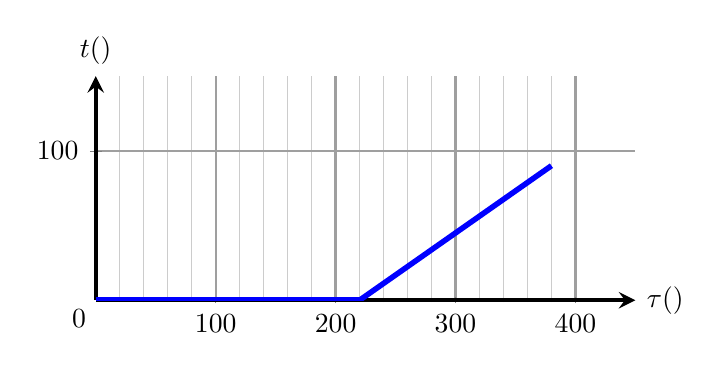
\begin{tikzpicture}  
			\begin{axis}[  ultra thick,yscale=0.5,
				xmin=0,  
				xmax=450,  
				xtick={0,100,200,300,400},
				ytick={0,100},
				minor x tick num=4,
				minor y tick num=0,
				ymin=0,  
				ymax=150, 
				samples=300,
				axis lines=center, 
				grid style={step=1, line width =0.4pt, color=gray!40!white},
				grid=both, %giới hạn ô lưới
				major grid style={line width=0.8pt,gray!75!white},
				xlabel=$\xsi{\tau}{\left(\si{\second}\right)}$, 		ylabel=$\xsi{t}{\left(\si{\celsius}\right)}$,
				every axis y label/.style={at=(current axis.above origin),anchor=south},  
				every axis x label/.style={at=(current axis.right of origin),anchor=west},  ]
				\addplot [line width=2pt, blue, smooth, domain=0:220] {0};  
				\addplot [line width=2pt, blue, smooth, domain=220:380] {0.5625*(x-220)}; 
				\coordinate (O) at (axis cs: 0,0);
			\end{axis}  
			\node[below left] at (O) {0};
		\end{tikzpicture}
	\end{center}
	\choiceTF[t]
	{\True Thời gian để nước đá tan hoàn toàn là $\SI{220}{\second}$}
	{\True Nếu hao phí nhiệt lượng là $\SI{2}{\percent}$, thì nhiệt nóng chảy riêng của nước đá là $\SI{334.18}{\kilo\joule/\kilogram}$}
	{Bỏ qua mọi hao phí thì nhiệt nóng chảy riêng của nước đá là $\SI{310}{\kilo\joule/\kilogram}$}
	{Trong giai đoạn từ thời điểm $\SI{0}{\second}$ đến $\SI{200}{\second}$, khối chất không nhận thêm nhiệt lượng}
	\loigiai{
		\begin{itemchoice}
			\itemch Đúng.
			\itemch Đúng. $H\calP t=m\lambda\Leftrightarrow 0,98\cdot930\cdot220=0,6\cdot\lambda\Rightarrow \lambda=\SI{334.18}{\kilo\joule/\kilogram}$.
			\itemch Sai. $\calP t=m\lambda\Leftrightarrow 930\cdot220=0,6\lambda\Rightarrow \lambda=\SI{341}{\kilo\joule/\kilogram}$.
			\itemch Sai. Từ thời điểm $\SI{0}{\second}$ đến $\SI{200}{\second}$, khối chất nhận nhiệt để nóng chảy.
		\end{itemchoice}
	}
\end{ex}
% ===================================================================
\begin{ex}
	Có hai chai nước lạnh A và B hoàn toàn giống nhau. Cho chai nước A vào chậu nước đến khi cân bằng nhiệt thì thấy nhiệt độ nước trong chậu giảm xuống. Lấy chai nước A ra ngoài và cho chai nước B vào chậu nước đến khi cân bằng nhiệt thì thấy nhiệt độ nước trong chậu tiếp tục giảm xuống, lấy chai B ra khỏi chậu nước. Xem như chỉ có sự trao đổi nhiệt giữa chai nước A, B và nước trong chậu.
	\choiceTF[t]
	{\True Sau khi lấy các chai nước ra khỏi chậu thì nhiệt độ của chai nước A cao hơn nhiệt độ của chai nước B}
	{Tổng độ tăng nhiệt độ của 2 chai nước bằng tổng độ giảm nhiệt độ của nước trong chậu ở 2 lần nhúng}
	{\True Độ giảm nhiệt độ của chậu nước trong lần nhúng chai nước A nhiều hơn lần nhúng chai nước	B}
	{Nhiệt lượng của chậu nước truyền cho hai chai nước là như nhau}
	\loigiai{
		\begin{itemchoice}
			\itemch Đúng.
			\begin{itemize}
				\item Thả chai nước A thì khi cân bằng nhiệt, nhiệt độ chai nước A bằng nhiệt độ $t_{\mathrm{cb1}}$ của nước trong chậu.
				\item Thả chai nước B thì khi cân bằng nhiệt, nhiệt độ chai nước B bằng nhiệt độ $t_{\mathrm{cb2}}$ của nước trong chậu.
				\item Mà nhiệt độ của nước trong chậu giảm xuống nên $t_{\mathrm{cb1}}>t_{\mathrm{cb2}}$.
			\end{itemize}
			\itemch Sai. Tổng độ tăng nội năng của 2 chai nước bằng tổng độ giảm nội năng của nước trong chậu.
			\itemch Đúng. \\
			$\begin{cases}
				m_Cc\left(t_C-t_1\right)=m_Ac\left(t_1-t_0\right)\\
				m_Cc\left(t_1-t_2\right)=m_Bc\left(t_2-t_0\right)
			\end{cases}\xrightarrow{m_A=m_B}\dfrac{t_C-t_1}{t_1-t_2}=\dfrac{t_1-t_0}{t_2-t_0}>1$.
			\itemch Sai. Nhiệt lượng chậu nước truyền cho chai A lớn hơn chai B.
		\end{itemchoice}
	}
\end{ex}
% ===================================================================
\begin{ex}
	Nhiệt kế rượu được chế tạo với thành phần chính của chất lỏng trong nhiệt kế là rượu. Một nhiệt kế rượu thông thường có giới hạn đo từ $\SI{-115}{\celsius}$ đến $\SI{78,5}{\celsius}$.
	\choiceTF[t]
	{\True Rượu được chọn làm nhiệt kế vì tính chất giãn nở đều theo nhiệt độ của nó}
	{\True Theo thang đo nhiệt độ Kelvin (làm tròn) thì giới hạn đo của nhiệt kế rượu kế trên là từ $\SI{158}{\kelvin}$ đến $\SI{351.5}{\kelvin}$}
	{Có thể dùng nhiệt kế rượu để đo nhiệt độ sôi của nước}
	{Hoàn toàn có thể dùng nước tinh khiết để thay thế cho rượu làm nhiệt kế}
	\loigiai{}
\end{ex}

\Closesolutionfile{ans}
\section{Câu trắc nghiệm trả lời ngắn} \textit{Thí sinh trả lời từ câu 1 đến câu 6}
\setcounter{ex}{0}
\Opensolutionfile{ans}[ans/G12-1-TL]
% ===============================================================
\begin{ex}
	Người ta cung cấp một nhiệt lượng $\SI{1.5}{\joule}$ cho chất khí đựng trong một xilanh đặt nằm ngang. Khí nở ra đẩy pittông di chuyển đều một đoạn $\SI{5}{\centi\meter}$. Biết lực ma sát giữa pittông và xilanh có độ lớn $\SI{20}{\newton}$. Xem như không có sự truyền nhiệt giữa khí và môi trường xung quanh. Tính độ biến thiên nội năng $\left(\si{\joule}\right)$ của khí trong xilanh?	
	\shortans{ 0,5}
	\loigiai{
		Công do khí thực hiện:
		$$A'=Fs=\left(\SI{20}{\newton}\right)\cdot\left(\SI{0.05}{\meter}\right)=\SI{1}{\joule}.$$
		Độ biến thiên nội năng của khí:
		$$\Delta U=Q+A=Q-A'=1,5-1=\SI{0.5}{\joule}.$$
	}
\end{ex}
% ===============================================================
\begin{ex}
	Một bình thuỷ tinh dung tích $\SI{20}{\liter}$ chứa $\SI{20}{\liter}$ khí oxygen. Nếu ta thêm vào bình $\SI{2}{\liter}$ khí oxygen nữa thì thể tích $\left(\si{\meter^3}\right)$ oxygen trong bình lúc này là bao nhiêu?
	\shortans{0,02 }
	\loigiai{
		Thể tích khí bằng thể tích bình chứa $V=\SI{20}{\liter}=\SI{0.02}{\meter^3}.$
	}
\end{ex}
% ===============================================================
\begin{ex}
	Rót khối lượng $m_{1}=\SI{0.5}{\kilogram}$ nước ở nhiệt độ $t_{1}=\SI{15}{\celsius}$ vào một bình nhiệt lượng kế có khối lượng $m_{2}=\SI{0.2}{\kilogram}$ đang ở nhiệt độ $t_{2}=\SI{30}{\celsius}$. Thả một cục nước đá có khối lượng $m_{3}=\SI{0.5}{\kilogram}$ ở nhiệt độ $t_{3}=\SI{-10}{\celsius}$ vào nước trong bình nhiệt lượng kế trên. Cho biết nhiệt dung riêng của nước, nước đá và bình nhiệt lượng kế tương ứng là $c_{1}=\SI{4.2E3}{\joule/\kilogram\cdot\kelvin}$; $c_{2}=\SI{2.1E3}{\joule/\kilogram\cdot\kelvin}$; $c_{3}=\SI{880}{\joule/\kilogram\cdot\kelvin}$; nhiệt nóng chảy của nước đá là $\lambda=\SI{3.3E5}{\joule/\kilogram}$. Bỏ qua sự trao đổi nhiệt với môi trường ngoài. Nhiệt độ $\left(\si{\celsius}\right)$ của hỗn hợp sau khi cân bằng nhiệt được thiết lập bằng bao nhiêu?
	\shortans{ 0}
	\loigiai{
		Nhiệt lượng nước và nhiệt lượng kế tỏa ra để giảm nhiệt độ xuống $\SI{0}{\celsius}$:
		$$Q_{\mathrm{tỏa}}=m_1c_1\left(t_1-0\right)+m_2c_3\left(t_2-0\right)=\SI{36.78}{\kilo\joule}.$$
		Nhiệt lượng nước đá thu vào để tăng nhiệt độ lên $\SI{0}{\celsius}$:
		$$Q_3=m_3c_2\left(0-t_3\right)=\SI{10.5}{\kilo\joule}.$$
		Nhiệt lượng nước đá cần thu vào để tan hoàn toàn:
		$$Q_{\mathrm{thu}}=m_3c_2\left(0-t_3\right)+m_3\lambda=\SI{175.5}{\kilo\joule}.$$
		Vì $Q_{\mathrm{thu}}>Q_{\mathrm{tỏa}}>Q_3$ nên nước đá chỉ tan một phần. Nhiệt độ cân bằng của hỗn hợp là $\SI{0}{\celsius}$.
		
	}
\end{ex}
% ===============================================================
\begin{ex}
	Người ta dùng bếp dầu hỏa để đun sôi nước, biết rằng phải tốn $\SI{150}{\gram}$ dầu hỏa mới đun sôi được $\SI{4.5}{\liter}$ nước ở $\SI{20}{\celsius}$, và cứ đốt $\SI{1}{\kilogram}$ dầu thì lượng nhiệt tỏa ra là $q=\SI{44E6}{\joule}$. Nhiệt dung riêng của nước là $\SI{4200}{\joule/\kilogram\cdot\kelvin}$, khối lượng riêng của nước là $\SI{1000}{\kilogram/\meter^3}$. Hiệu suất $\left(\si{\percent}\right)$ của bếp là bao nhiêu? (làm tròn đến 1 chữ số sau dấu phẩy)
	\shortans{22,9 }
	\loigiai{
		$$H=\dfrac{m_nc\Delta t}{m_dq}=\dfrac{DVc\Delta t}{m_dq}\approx\SI{22.9}{\percent}.$$
	}
\end{ex}
% ===============================================================
\begin{ex}
	Tại một đập thủy điện, người ta cho nước rơi từ độ cao $\SI{96}{\meter}$ xuống và đập vào cánh tuabin làm quay máy phát điện, biết rằng $\SI{50}{\percent}$ thế năng của nước làm nước nóng lên. Cho biết nhiệt dung riêng của nước là $\SI{4190}{\joule/\kilogram\cdot\kelvin}$. Lấy $g=\SI{10}{\meter/\second^2}$. Độ biến thiên nhiệt độ $\left(\si{\kelvin}\right)$ của nước là bao nhiêu? (làm tròn đến 1 chữ số sau dấu phẩy)
	\shortans{0,1 }
	\loigiai{
		$$\Delta t=\dfrac{mghH}{mc}=\dfrac{10\cdot96\cdot0,5}{4190}\approx\SI{0.1}{\kelvin}.$$
	}
\end{ex}
% ===============================================================
\begin{ex}
	Sự biến thiên nhiệt độ của khối nước đá đựng trong ca nhôm theo nhiệt lượng cung cấp được cho trên đồ thị. Cho nhiệt dung riêng của nước và nhôm lần lượt là $c_{1}=\SI{4200}{\joule/\kilogram\cdot\kelvin}$; $c_{2}=\SI{880}{\joule/\kilogram\cdot\kelvin}$, nhiệt nóng chảy của nước đá là $\lambda=\SI{3.4E5}{\joule/\kilogram}$. Khối lượng của ca nhôm bằng bao nhiêu $\si{\gram}$ (làm tròn đến phần nguyên)?
	\begin{center}
		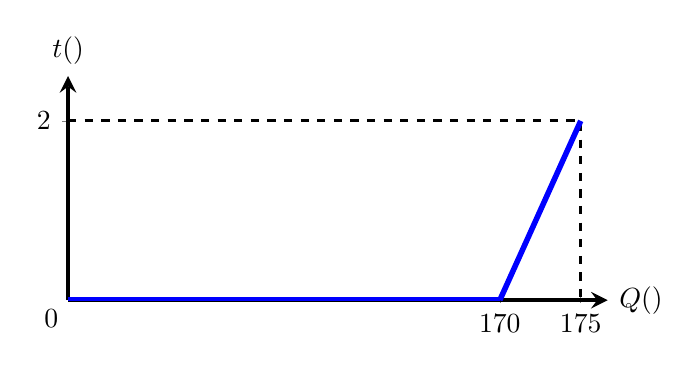
\begin{tikzpicture}  
			\begin{axis}[  ultra thick,yscale=0.5,
				xmin=0,  
				xmax=10,  
				xtick={0,8,9.5},
				ytick={0,2},
				ymin=0,  
				ymax=2.5, 
				samples=300,
				xticklabels={0,170,175},
				axis lines=center, 
				xlabel=$\xsi{Q}{\left(\si{\kilo\joule}\right)}$, 		ylabel=$\xsi{t}{\left(\si{\celsius}\right)}$,
				every axis y label/.style={at=(current axis.above origin),anchor=south},  
				every axis x label/.style={at=(current axis.right of origin),anchor=west},  ]
				\draw[dashed, line width=1pt] (axis cs: 0,2)--(axis cs: 9.5,2)--(axis cs: 9.5,0);
				\addplot [line width=2pt, blue, smooth, domain=0:8] {0};  
				\addplot [line width=2pt, blue, smooth, domain=8:9.5] {4*(x-8)/3};  
				\coordinate (O) at (0,0);
			\end{axis} 
			\node[below left] at (O) {0}; 
		\end{tikzpicture}
	\end{center}
	\shortans{455 }
	\loigiai{
		Khối lượng nước đá:
		$m_{\text{đ}}=\dfrac{\SI{170E3}{\joule}}{\lambda}=\SI{0.5}{\kilogram}.$\\
		Trong giai đoạn hệ tăng nhiệt độ:
		$$\left(m_{\text{đ}}c_1+mc_2\right)\cdot\Delta t=\SI{5E3}{\joule}\Rightarrow m\approx\SI{0.455}{\kilogram}=\SI{455}{\gram}.$$
	}
\end{ex}
\Closesolutionfile{ans}
\begin{center}
	\textbf{-- HẾT --}
\end{center}








